% !TEX root = PREN2_Dokumentation.tex
\section{System-Spezifikation}\label{SystemSpezifikation}
\subsection{Systemübersicht}
\subsubsection{Systemarchitektur}
\begin{figure}[H]
    \centering
    \includegraphics[width=1\textwidth]{images/systemoverview.png}
    \caption[Systemarchitektur]{Systemarchitektur,\\ Quelle: Autoren}
    \label{img: Systemarchitektur des Projektes}
\end{figure}
\newpage
\subsubsection{Kontextdiagram}\label{Kontextdiagram}
\begin{figure}[H]
    \centering
   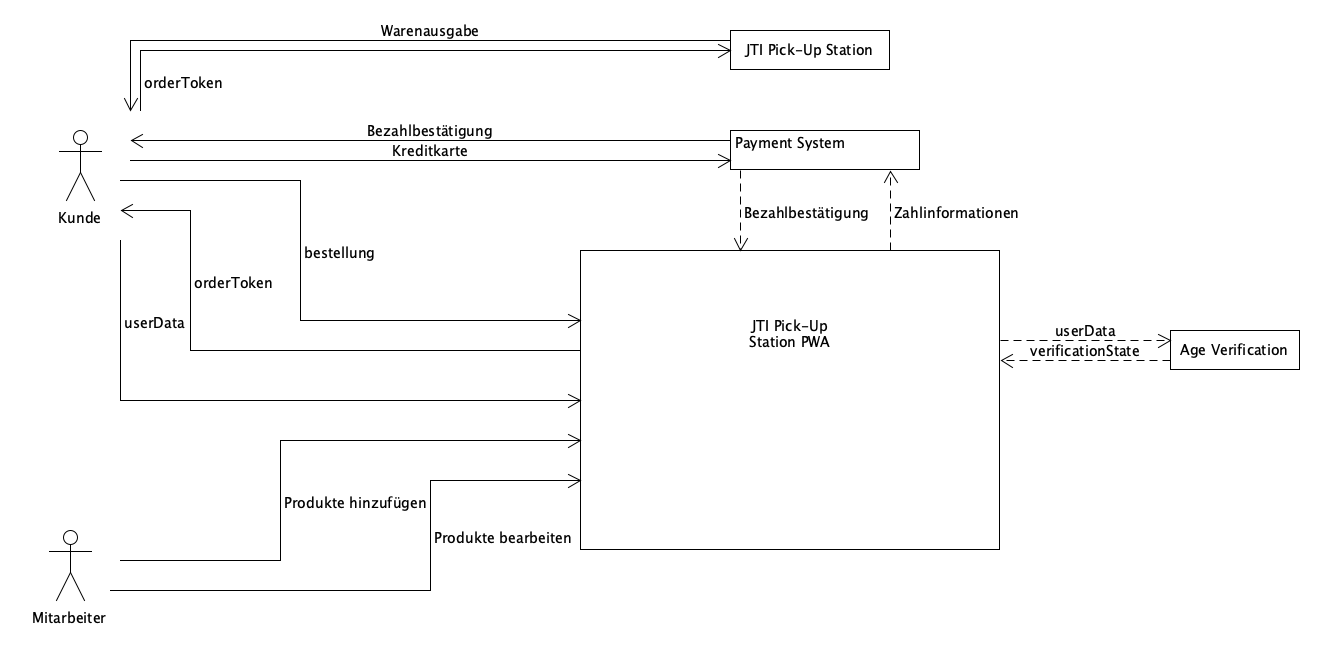
\includegraphics[width=1\textwidth]{images/kontextdiagramm.png}
    \caption[Kontextdiagramm]{Kontextdiagramm,\\ Quelle: Autoren}
    \label{img: Kontextdiagramm des Projektes}
\end{figure}
\newpage


\newpage
\subsection{Architektur und Designentscheide}
Es wurde bei diesem Projekt auf eine REST-Architektur gesetzt. Die Web-Applikation wird als \ac{PWA} umgesetzt. 
\subsubsection{Modelle und Sichten}
In diesem Projekt wird zwischen zwei verschiedenen Sichten unterschieden:
\begin{itemize}
    \item \textbf{Kunde} Es handelt sich dabei um die Person, welche in der \ac{PWA} Produkte bestellt und diese anschliessend abholt. 
    \item \textbf{Administrator} Dem Administrator ist es möglich, Produkt hinzuzufügen, zu verändern oder auch zu löschen. 
    \item \textbf{Programmierer: } Dieser konzipiert und realisiert die Applikation gemäss den Anforderungen des Auftraggebers.
\end{itemize}
\subsubsection{Daten (Mengengerüst und Strukturen)}
\paragraph{Datenbankschema}
Das Datenbankschema wurde mittels Reverse Engineering mit MySQL Workbench erstellt und ist in der Abbildung \ref{img: datebankschema} ersichtlich.
\begin{figure}[H]
    \centering
    %\includegraphics[width=1\textwidth]{bilder/datenbankschema.png}
    \caption[Datenbankschema]{Datenbankschema, Quelle: Autoren}
    \label{img: datebankschema}
\end{figure}
\subsubsection{Entwurfsentscheide}
\paragraph{Frontend}
\subparagraph{Technologien}

\subparagraph{Projektstruktur}
\paragraph{Backend}
\subparagraph{Spring Boot}
Für die Backendentwicklung wurde Spring Boot in der Version 2.3.4 genutzt.
\paragraph{Datenbank}
\paragraph{Konfigurationen}
\subparagraph{Frontend}

\newpage
\subparagraph{Backend}
\newpage
\subsection{Schnittstellen}

\subsubsection{Externe Schnittstellen}
\paragraph{REST API}

\subsubsection{Wichtige interne Schnittstellen}


\paragraph{Schnittstelle}
\subparagraph{Steckbrief}

\subparagraph{Einsatz, Abläufe, Voraussetzungen und Zusicherung}

\subparagraph{Aufbau und Konfiguration}

\subparagraph{Fehlerbehandlung}

\subparagraph{Qualitätsmerkmale}
\subparagraph{Entwurfsentscheidungen}

\subparagraph{Beispielverwendung}

\subsubsection{Benutzerschnittstellen}

\subsection{Environment-Anforderungen}\label{environmentanforderungen}

\subsubsection{Hardware}
Folgende Hardware wurde für diese Applikation verwendet und kann als ausreichend betrachtet werden:

\subsubsection{Software}

\begin{itemize}

\end{itemize}
\newpage